\documentclass[tikz,border=1.8mm]{standalone}

\definecolor{fvmadaptedge}{HTML}{8A7E7E}
\definecolor{externalface}{HTML}{8FB9E8}
\definecolor{nodefill}{HTML}{FFFFFF}
\usetikzlibrary{arrows.meta}

\begin{document}
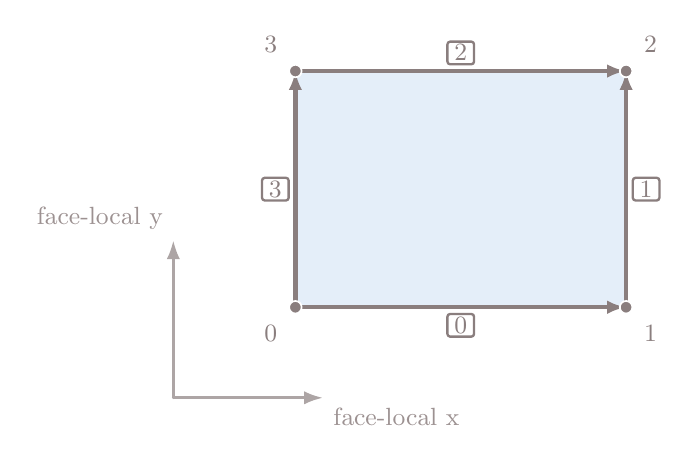
\begin{tikzpicture}[
  line join=round,
  line cap=round,
  face/.style={fill=externalface,fill opacity=0.24,draw=none},
  edgearrow/.style={draw=fvmadaptedge,line width=0.55mm,-{Latex[length=2.4mm,width=1.7mm]}},
  axis/.style={draw=fvmadaptedge!70,line width=0.34mm,-{Latex[length=2.4mm,width=1.7mm]}},
  vertex/.style={fill=fvmadaptedge,draw=white,line width=0.22mm,circle,inner sep=1.6pt},
  nodelabel/.style={font=\small,text=fvmadaptedge},
  edgenum/.style={rectangle,rounded corners=1.0pt,draw=fvmadaptedge,line width=0.30mm,fill=nodefill,inner xsep=2.5pt,inner ysep=1.2pt,font=\small,text=fvmadaptedge},
  axislabel/.style={font=\small,text=fvmadaptedge!85}
]
  \coordinate (N0) at (0,0);
  \coordinate (N1) at (4.2,0);
  \coordinate (N2) at (4.2,3.0);
  \coordinate (N3) at (0,3.0);

  \path[face] (N0) -- (N1) -- (N2) -- (N3) -- cycle;

  \draw[edgearrow] (N0) -- (N1);
  \draw[edgearrow] (N1) -- (N2);
  \draw[edgearrow] (N3) -- (N2);
  \draw[edgearrow] (N0) -- (N3);

  \node[edgenum,below=2pt] at (2.1,0) {0};
  \node[edgenum,right=2pt] at (4.2,1.5) {1};
  \node[edgenum,above=2pt] at (2.1,3.0) {2};
  \node[edgenum,left=2pt] at (0,1.5) {3};

  \foreach \p in {N0,N1,N2,N3} {
    \node[vertex] at (\p) {};
  }

  \node[nodelabel,below left=3pt] at (N0) {0};
  \node[nodelabel,below right=3pt] at (N1) {1};
  \node[nodelabel,above right=3pt] at (N2) {2};
  \node[nodelabel,above left=3pt] at (N3) {3};

  \draw[axis] (-1.55,-1.15) -- (0.35,-1.15)
    node[axislabel,below right] {face-local x};
  \draw[axis] (-1.55,-1.15) -- (-1.55,0.85)
    node[axislabel,above left] {face-local y};
\end{tikzpicture}
\end{document}
